\documentclass[a4paper]{article}

\iffalse
\usepackage[L7x,T1]{fontenc}
\usepackage[lithuanian]{babel}
\else
\usepackage[T1]{fontenc}
\usepackage[english]{babel}
\fi

\usepackage[utf8]{inputenc}
\usepackage{a4wide}
\usepackage{csquotes}
\usepackage[maxbibnames=99,style=authoryear]{biblatex}
\usepackage[pdfusetitle]{hyperref}
\usepackage{enumitem}
\usepackage[toc,page,title]{appendix}
\addbibresource{bib.bib}
\usepackage{caption}
\usepackage{subcaption}
\usepackage{gensymb}
\usepackage{varwidth}
\usepackage{tabularx}
\usepackage{float}
\usepackage{tikz}
\usepackage{minted}
\usetikzlibrary{er,positioning}
\definecolor{mypurple}{RGB}{117,112,179}
\input{version}

\newcommand{\DP}{Douglas \& Peucker}
\newcommand{\VW}{Visvalingam--Whyatt}
\newcommand{\WM}{Wang--M{\"u}ller}

\title{
    Cartografic Generalization of Lines using free software \\
    (example of rivers) \\ \vspace{4mm}
}

\iffalse
https://bost.ocks.org/mike/simplify/
http://bl.ocks.org/msbarry/9152218

small scale: 1:XXXXXX
large scale: 1:XXX

a4: 210x297mm
a5: 148x210mm
a6: 105x148xmm
a7: 74x105mm
a8: 52x74mm

Crossing:
Xmin: 623306
Ymin: 6109635
Xmax: 625526
Ymax: 6111210
623306 6109635 625526 6111210
Crossing wxh: 2220, 1575 (m)


connect rivers first to a single polylines:
- some algs can preserve connectivity, some not.

ideal hypothesis: mueller algorithm + topology may fully realize cartographic generalization tasks.

what scales and what distances?

= Intro: Aktualumas
FOSS nėra realizuotas tinkamas kartografinio realizavimo algoritmas (2–3 sakiniai). Kad kartografai turėtų
įrankį upių generalizavimui.

Bazė: imame tai, ką dabar turi kartografai įrankių paletėj.

Imti mažus upės vingius. Paimti mažas atkarpėles ir palyginti su originalia.
Todėl, kad nėra kilpų.

Zeimena extents: [606922,6097557,627230,6126362]
20308 x 28805 (w x h)

\fi

\author{Motiejus Jakštys}

\date{
    \vspace{10mm}
    Version: \VCDescribe \\ \vspace{4mm}
    Generated At: \GeneratedAt
}

\begin{document}
\maketitle

\begin{abstract}
\label{sec:abstract}
Current open-source line generalization solutions have their roots in
    mathematics and geometry, thus emit poor cartographic output. Therefore, if
    one is using open-source technology to generalize cartographic objects,
    their downscaled counterparts will be incorrectly scale-adjusted. This
    paper explores the available down-scaling implementations, highlights some
    of their deficiencies, and suggests a viable algorithm for an avid GIS
    developer. Once the new algorithm becomes usable from within open-source
    GIS software (e.g. QGIS or PostGIS), small-scale maps created by free
    software will have a chance to be of higher quality.
\end{abstract}

\newpage

\tableofcontents
\listoffigures

\newpage

\section{Introduction}
\label{sec:introduction}

A number of cartographic line generalization algorithms have been researched,
which claim to better process cartographic objects like lines. These fall into
two rough categories:
\begin{itemize}
    \item Cartographic knowledge was encoded to an algorithm (bottom-up
        approach). One among these are \cite{wang1998line}.
    \item Mathematical shape transformation which yields a more
        cartographically suitable down-scaling. E.g. \cite{jiang2003line},
        \cite{dyken2009simultaneous}, \cite{mustafa2006dynamic},
        \cite{nollenburg2008morphing}.
\end{itemize}

During research for the mentioned articles, prototype code has been written for
most of the algorithms. However, none of them seem to be available for use
except for the two "classical" ones -- {\DP} and {\VW}.

\cite{wang1998line} is an algorithm specifically created for cartographic
generalization and available for general use, though it is only currently
available in a commercial product. This poses a problem for map creation in
open source software: there is not a similar high-quality simplification
algorithm to create down-scaled maps, so any cartographic work, which uses line
generalization as part of its processing, will be of sub-par quality.
We believe that availability of high-quality open-source tools is an important
foundation for future cartographic experimentation and development, thus it
it benefits the cartographic society as a whole.

This paper will be reviewing and comparing two widely available algorithms that
are often used for line generalization:
\begin{itemize}
    \item \cite{douglas1973algorithms} via
        \href{https://postgis.net/docs/ST_Simplify.html}{PostGIS Simplify}.

    \item \cite{visvalingam1993line} via
        \href{https://postgis.net/docs/ST_SimplifyVW.html}{PostGIS SimplifyVW}.

\end{itemize}

Since both algorithms produce jaggy output lines, it is worthwhile to process
those through a widely available \cite{chaikin1974algorithm} smoothing
algorithm via \href{https://postgis.net/docs/ST_ChaikinSmoothing.html}{PostGIS
ChaikinSmoothing}.

Review of the available algorithms will be followed by desiderata for a
possible open-source addition. In the end, we will issue a recommendation,
which algorithm can be picked up and implemented by an avid GIS developer.

\section{Visual comparison}

Lakaja and large part of Žeimena (see figure~\ref{fig:zeimena} on
page~\pageref{fig:zeimena}) will be used as inputs to the generalization
algorithms, because the river exhibits both both straight and curved shape, is
a combination of two curly rivers, and author's familiarity with the location.

Since the map area is large (approx. 20km by 28km, scale $1:300 000$), we will
also review a subset of the area of approx 2200m by 1575m. The zoomed-in
version will help explain some of the deficiencies in the reviewed algorithms.

\begin{figure}[H]
    \centering
    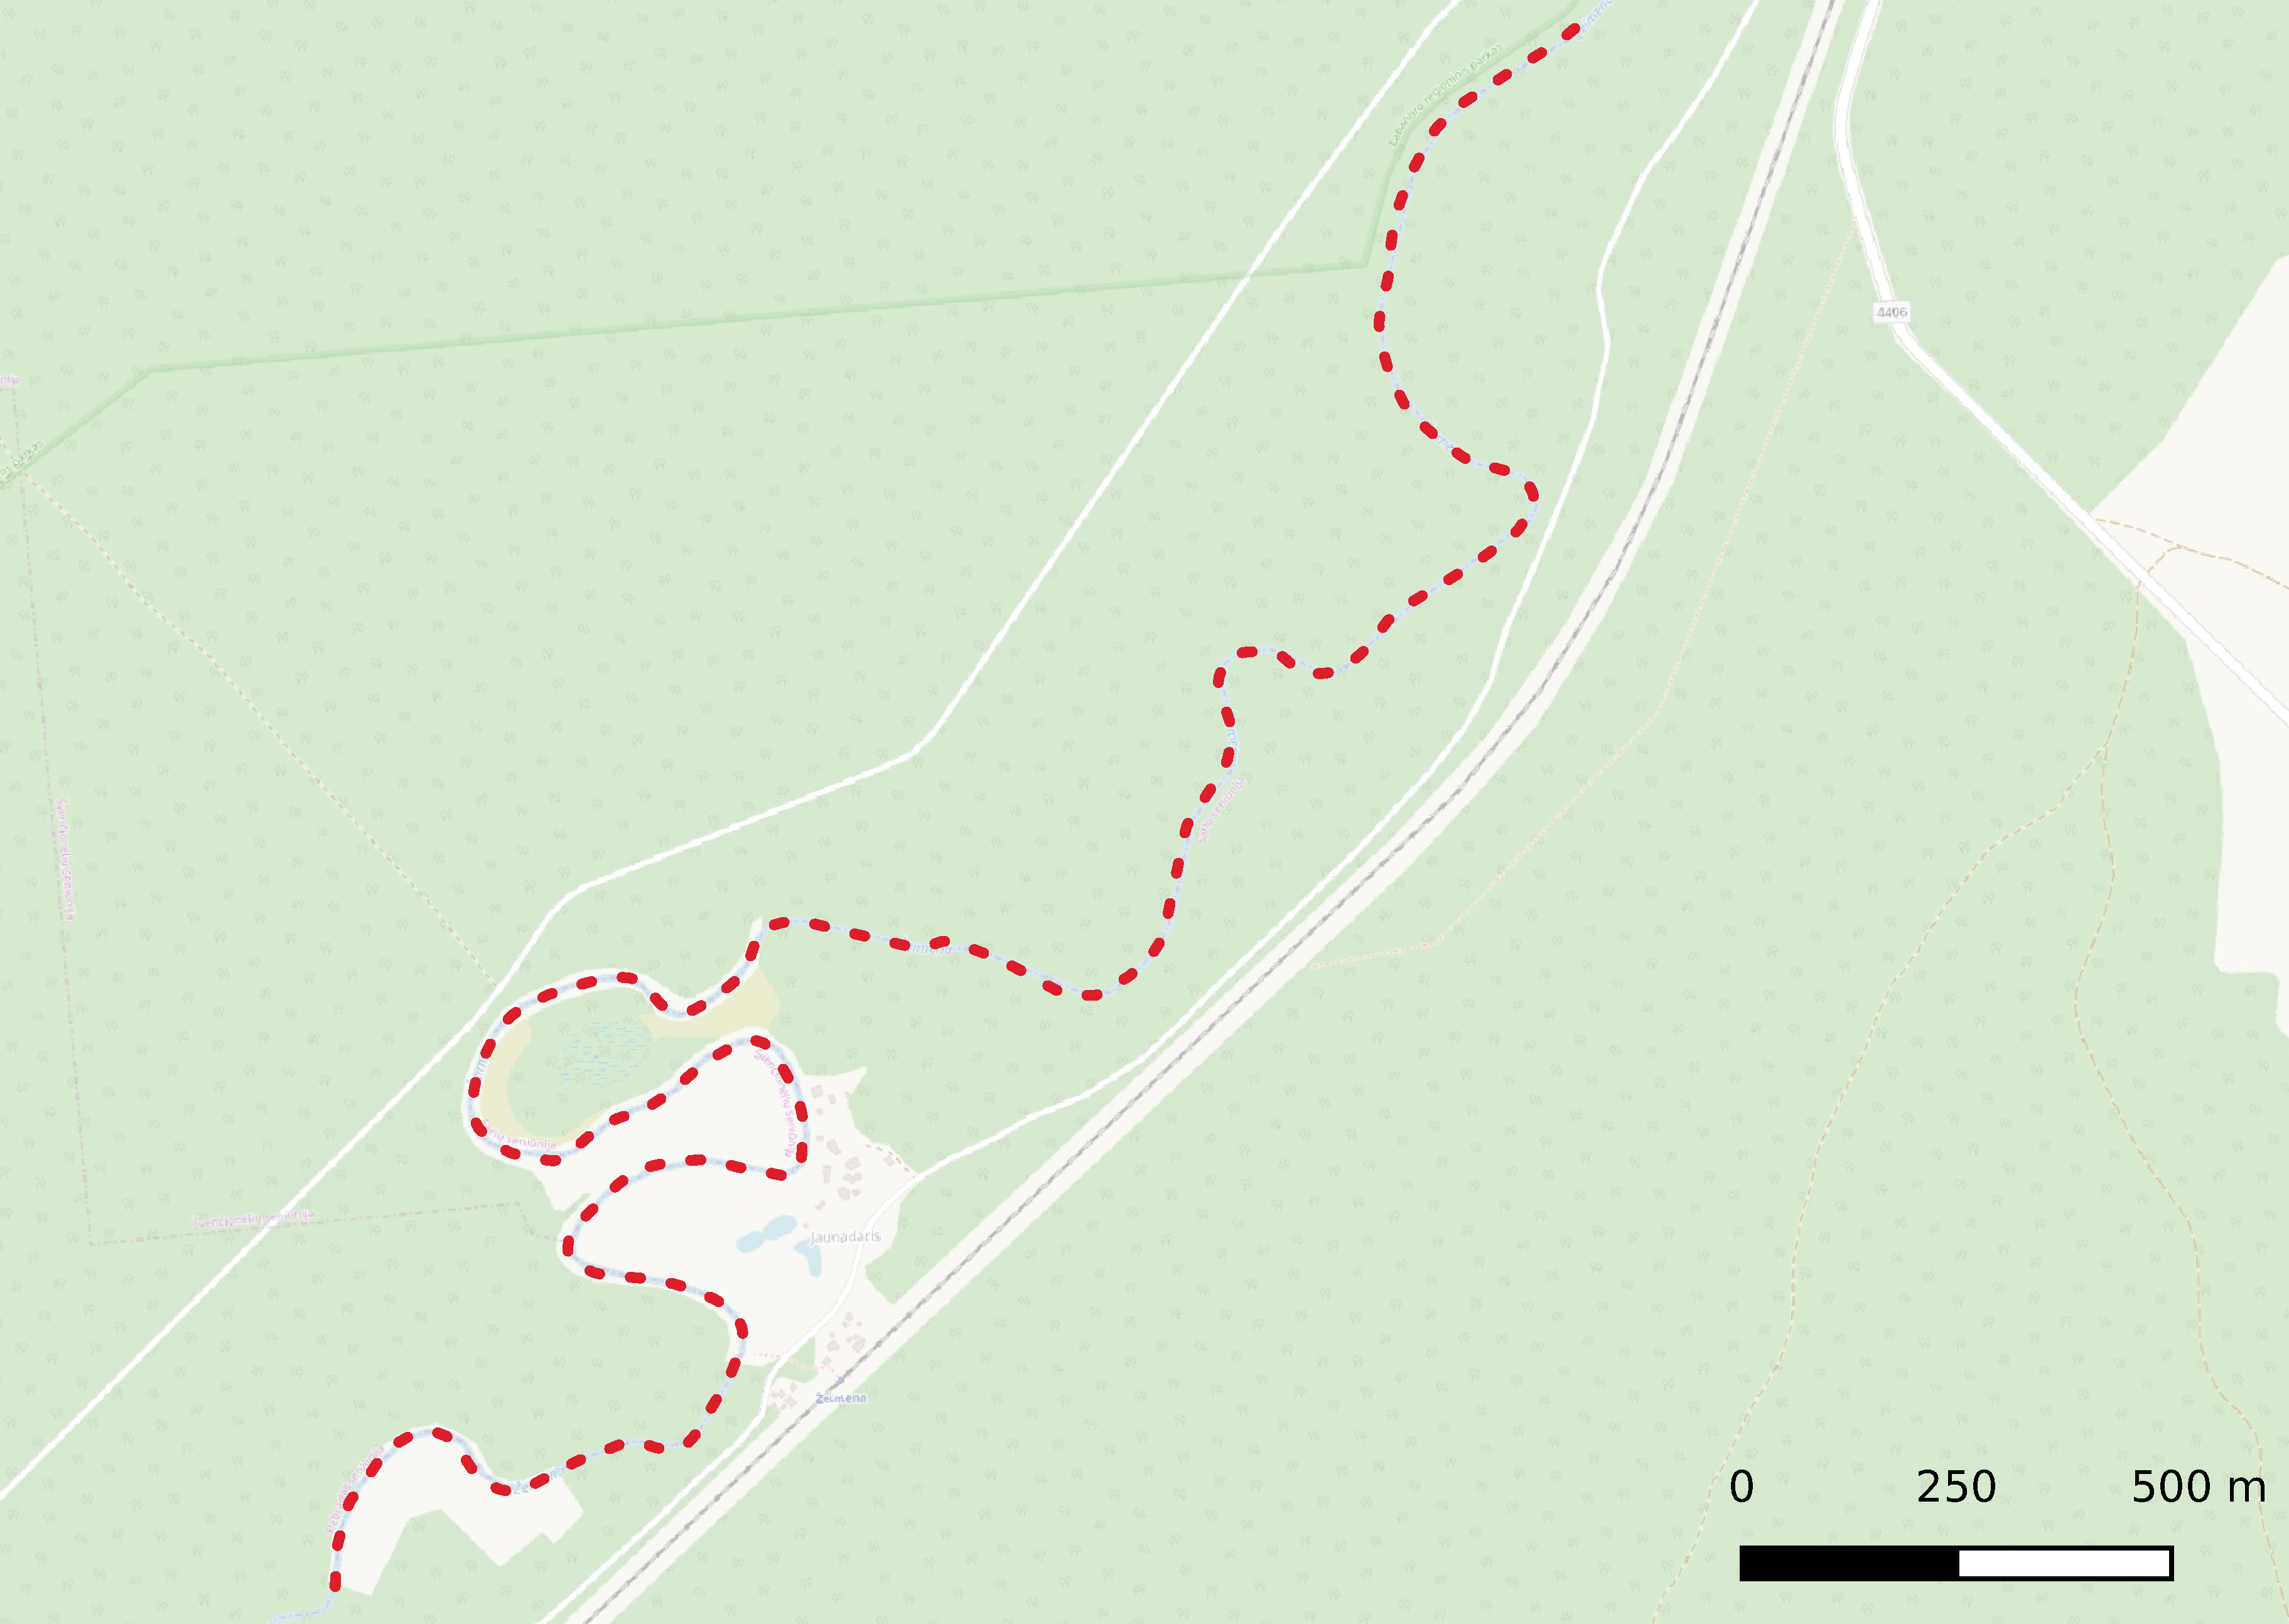
\includegraphics[width=67.5mm]{zeimena}
    \caption{Lakaja and Žeimena, with marked river crossing area, $1:300 000$}
    \label{fig:zeimena}
\end{figure}

\begin{figure}[h]
    \centering
    \includegraphics[width=74mm]{crossing}
    \caption{River crossing area zoomed in, $1:30 000$}
    \label{fig:crossing}
\end{figure}

To visually evaluate the Žeimena sample, examples for {\DP} and {\VW}
were created using the following parameters:

\begin{enumerate}[label=(\Roman*)]
    \item {\DP} tolerance: $tolerance := 125 * 2^n, n = 0,1,...,5$.
    \item {\VW} tolerance: $vwtolerance = tolerance ^ 2$\label{itm:2}.
\end{enumerate}

Parameter~\ref{itm:2} requires explanation. Tolerance for {\DP} is specified in
linear units, in this case, meters. Tolerance for {\VW} is specified in area
units $m^2$. As author was not able to locate formal comparisons between the
two (i.e. how to calculate one tolerance value from the other, so the results
are comparable?), {\DP} tolerance was arbitrarily squared and fed to {\VW}. To
author's eye, this provides comparable and reasonable results, though could be
researched.

As can be observed in table~\ref{tab:comparison-zeimena} on
page~\pageref{tab:comparison-zeimena}, both simplication algorithms convert
bends to chopped lines. This is especially visible in tolerances 256 and 512.
In a more robust simplification algorithm, the larger tolerance, the larger the
bends on the original map should be retained.

\begin{figure}[H]
    \renewcommand{\tabularxcolumn}[1]{>{\center\small}m{#1}}
    \begin{tabularx}{\textwidth}{ p{2.1cm} | X | X | }
        Tolerance DP/VW                                                   &
        Douglas \& Peucker                                                &
        Visvalingam-Whyatt                                                \tabularnewline \hline

        128/16384                                                         &
        \includegraphics[width=\linewidth]{zeimena_douglas_128}           &
        \includegraphics[width=\linewidth]{zeimena_visvalingam_128}       \tabularnewline \hline

        256/65536                                                         &
        \includegraphics[width=.5\linewidth]{zeimena_douglas_256}         &
        \includegraphics[width=.5\linewidth]{zeimena_visvalingam_256}     \tabularnewline \hline

        512/262144                                                        &
        \includegraphics[width=.25\linewidth]{zeimena_douglas_512}        &
        \includegraphics[width=.25\linewidth]{zeimena_visvalingam_512}    \tabularnewline \hline

        1024/1048576                                                      &
        \includegraphics[width=.125\linewidth]{zeimena_douglas_1024}      &
        \includegraphics[width=.125\linewidth]{zeimena_visvalingam_1024}  \tabularnewline \hline

        2048/4194304                                                      &
        \includegraphics[width=.0625\linewidth]{zeimena_douglas_2048}     &
        \includegraphics[width=.0625\linewidth]{zeimena_visvalingam_2048} \tabularnewline \hline

        4096/16777216                                                     &
        \includegraphics[width=.0625\linewidth]{zeimena_douglas_4096}     &
        \includegraphics[width=.0625\linewidth]{zeimena_visvalingam_4096} \tabularnewline \hline
    \end{tabularx}
    \caption{{\DP} and {\VW} on Žeimena}
    \label{tab:comparison-zeimena}
\end{figure}

To ease the discussion on shapes in the resulting output, it is useful to
define what a "blunt bend" is: it is a river bent that looks like a cutout from
a large circle, ilustrated in figure~\ref{fig:blunt-bent}.

\begin{figure}[h]
    \centering
    \begin{tikzpicture}
        \draw[color=mypurple] (-5,0) -- (-3, 0) ;
        \draw[color=mypurple] (0,0) arc (60:120:3) ;
        \draw[color=mypurple] (0,0) -- (2, 0) ;
    \end{tikzpicture}
    \caption{Blunt bent}
    \label{fig:blunt-bent}
\end{figure}

Once zoomed in to the river crossing area with {\DP} and {\VW} applied, it
becomes apparent that both large blunts are normalized to single lines, the
shape becomes jagged and unpleasant for the eye. See
table~\ref{tab:comparison-crossing} on page~\pageref{tab:comparison-crossing}.

\begin{figure}[h]
    \renewcommand{\tabularxcolumn}[1]{>{\center\small}m{#1}}
    \begin{tabularx}{\textwidth}{ p{2.1cm} | X | X | }
        Tolerance DP/VW                                                      &
        Douglas \& Peucker                                                   &
        Visvalingam-Whyatt                                                   \tabularnewline \hline

        64/4096                                                              &
        \includegraphics[width=\linewidth]{overlaid_zeimena_douglas_64}      &
        \includegraphics[width=\linewidth]{overlaid_zeimena_visvalingam_64}  \tabularnewline \hline

        128/16384                                                            &
        \includegraphics[width=\linewidth]{overlaid_zeimena_douglas_128}     &
        \includegraphics[width=\linewidth]{overlaid_zeimena_visvalingam_128} \tabularnewline \hline

        256/65536                                                            &
        \includegraphics[width=\linewidth]{overlaid_zeimena_douglas_256}     &
        \includegraphics[width=\linewidth]{overlaid_zeimena_visvalingam_256} \tabularnewline \hline

    \end{tabularx}
    \caption{{\DP} and {\VW} on river crossing area}
    \label{tab:comparison-crossing}
\end{figure}

As the reader may observe, the output lines, especially with higher tolerances,
are jaggy. Higher-tolerance jaggy outputs from {\VW} and {\DP}, passed through Chaikin,
are displayed in table~\ref{tab:chaikin-crossing} on
page~\page{tab:chaikin-crossing}.

\begin{figure}[h]
    \renewcommand{\tabularxcolumn}[1]{>{\center\small}m{#1}}
    \begin{tabularx}{\textwidth}{ p{2.1cm} | X | X | }
        Tolerance DP/VW                                                              &
        Douglas \& Peucker                                                           &
        Visvalingam-Whyatt                                                           \tabularnewline \hline

        128/16384                                                                    &
        \includegraphics[width=\linewidth]{chaikin_overlaid_zeimena_douglas_128}     &
        \includegraphics[width=\linewidth]{chaikin_overlaid_zeimena_visvalingam_128} \tabularnewline \hline

        256/65536                                                                    &
        \includegraphics[width=\linewidth]{chaikin_overlaid_zeimena_douglas_256}     &
        \includegraphics[width=\linewidth]{chaikin_overlaid_zeimena_visvalingam_256} \tabularnewline \hline

    \end{tabularx}
    \caption{Chaikin-smoothened {\DP} and {\VW} on river crossing area}
    \label{tab:chaikin-crossing}
\end{figure}

There is another issue on the wishlist beyond jaggyness and loss of large bents
-- combining close bends to larger ones.

\subsection{Combining bends}

Imagine there are two small bends close to each other, similar to
figure~\ref{fig:sinewave2} on page~\pageref{fig:sinewave2}, and one needs to
generalize it. The bends are too large to ignore replace them with a straight
line, but too small to retain both and retain their complexity.

According to cartographic generalization rules
(\cite{miuller1995generalization}), consecutive small bends should be combined
into larger bends. {\WM} encoded this process to an algorithm.

\begin{figure}[h]
    \centering
    \includegraphics[width=52mm]{sinewave2}
    \caption{Example river bend that should be generalized}
    \label{fig:sinewave2}
\end{figure}

When one applies {\DP} to figure~\ref{fig:sinewave2}, either both bends remain,
or become a straight line, see table~\ref{tab:comparison-sinewave2} on
page~\pageref{tab:comparison-sinewave2}.

\begin{figure}[h]
    \renewcommand{\tabularxcolumn}[1]{>{\center\small}m{#1}}
    \begin{tabularx}{\textwidth}{ p{1.5cm} | X | X | }
        Tolerance DP/VW                                                       &
        Douglas \& Peucker                                                    &
        Visvalingam-Whyatt                                                    \tabularnewline \hline

        2/4                                                                   &
        \includegraphics[width=\linewidth]{overlaid_sinewave2_douglas_2}      &
        \includegraphics[width=\linewidth]{overlaid_sinewave2_visvalingam_2}  \tabularnewline \hline

        16/256                                                                &
        \includegraphics[width=\linewidth]{overlaid_sinewave2_douglas_16}     &
        \includegraphics[width=\linewidth]{overlaid_sinewave2_visvalingam_16} \tabularnewline \hline

        32/1024                                                               &
        \includegraphics[width=\linewidth]{overlaid_sinewave2_douglas_32}     &
        \includegraphics[width=\linewidth]{overlaid_sinewave2_visvalingam_32} \tabularnewline \hline

    \end{tabularx}
    \caption{{\DP} and {\VW} on example wave}
    \label{tab:comparison-sinewave2}
\end{figure}

Ideally, the double-bend in figure~\ref{fig:sinewave2} should be normalized to
a larger single-bend, similar to figure~\ref{fig:sinewave1} on
page~\pageref{fig:sinewave2}.

\begin{figure}[h]
    \centering
    \includegraphics[width=52mm]{sinewave1}
    \caption{Desired river bend generalization}
    \label{fig:sinewave1}
\end{figure}

To recap, both {\VW} and {\DP} simplify the lines, but their cartographic
output, when zoomed in, looks poorly to the human eye. Can a better solution be
found?

\section{Recommendation}
\label{sec:recommendation}

So far, we have reviewed two widely available open-source generalization
algorithms {\DP} and {\VW}, and now can enumerate the shortcomings:
\begin{itemize}
    \item Resulting generalized lines look jaggy and, when zoomed in,
        unpleasant to the eye.
    \item Blunt bends are generalized to straight lines, even though sometimes
        they should remain blunt bends (or even exhagerated bends).
    \item Consecutive small bends should be normalized into a larger bend.
\end{itemize}

According to \cite{wang1998line}, their algorithm fixes all 3 issues above. The
algorithm is relatively simple to understand for a non-expert cartographer
software developer, and thus should be feasible to implement in a few weeks.

\section{Conclusions}
\label{sec:conclusions}

We have evaluated two readily available line simplification algorithms using a
river sample and a synthetic bend: {\VW} and {\DP}. Once looking at the
examples, it is quite easy to see the most glaring deficiencies when applying
those two for comparing cartographic generalization.

We are suggesting to complement open-source list of
available algorithms with {\WM}, which was created for cartographic
generalization, and should fix the shortcomings identified in this paper.

\section{Related Work and future suggestions}
\label{sec:related_work}

\cite{stanislawski2012automated} studied different types of metric assessments,
such as Hausdorff distance, segment length, vector shift, surface displacement,
and tortuosity for the generalization of linear geographic elements. This
research can provide references to the appropriate settings of the line
generalization parameters for the maps at various scales.

As noted in parameter~\ref{itm:2} on page~\pageref{itm:2}, it would be useful
to have a formula mapping {\DP} tolerance to {\VW}. That way, visual
comparisons between line simplification algorithms could be more objective.

\printbibliography

\begin{appendices}

\section{Žeimena and Lakaja in context}

\begin{figure}[H]
    \centering
    \includegraphics[width=148mm]{zeimena-pretty}
    \caption{Lakaja and Žeimena river in context}
\end{figure}

\section{Code listings}

For the curious users it may be useful to see how the analysis was executed.
Also, given the source listings, it should be relatively straightforward to
re-run the same analysis on a different area.

The input files outside of these listings are {\tt zeimena.gpkg}, which is a
manually created GeoPackage containing Žeimena and Lakaja rivers, and the
\LaTeX\ report itself.

The analysis was executed and report was generated on Ubuntu 20.04 with only
system packages. This should be sufficient: {\tt postgis gdal-bin biber
latexmk texlive-bibtex-extra python3-geopandas python3-pygments}.

\subsection{douglas.sql}
Transforms a layer ({\tt :src}) to {\DP} using $tolerance$ tolerance into
{\tt :tbl} table.
\inputminted[fontsize=\small]{sql}{douglas.sql}

\subsection{visvalingam.sql}
Transforms a layer ({\tt :src}) to {\VW} using $tolerance^2$ tolerance into
{\tt :tbl} table.
\inputminted[fontsize=\small]{sql}{visvalingam.sql}

\subsection{fig2layer.py}
Creates figures (square, sine wave) as geopackage files.
\inputminted[fontsize=\small]{python}{fig2layer.py}

\subsection{Makefile}
This file binds all the pieces together:
\begin{itemize}
    \item Prepares the PostGIS database.
    \item Generates helper figures (sine waves, squares).
    \item Runs analysis on input files ({\DP} and {\VW}).
    \item Invokes {\tt latexmk} as a final report generation step.
\end{itemize}
\inputminted[fontsize=\small]{make}{Makefile}

\subsection{layer2img.py}
This file accepts a layer (or two) and generates a PDF image suitable for embedding into the report.
\inputminted[fontsize=\small]{python}{layer2img.py}

\subsection{managedb}
Manages a PostGIS database in the project directory. That way, the database can
be torn down and re-created by automated tools like the {\tt Makefile} itself.
You may need to update the paths in this script to suit your environment.
\inputminted[fontsize=\small]{bash}{managedb}

\end{appendices}
\end{document}
